\documentclass[11pt,a4paper]{scrartcl}

%------------------------------------------%

\usepackage[utf8]{inputenc}
\usepackage[german]{babel}
\usepackage{amsmath}
\usepackage{amsfonts}
\usepackage{amssymb}
\usepackage{booktabs}
\usepackage{graphicx}
\usepackage{float}
%\usepackage{gnuplot-lua-tikz}
\usepackage{hyperref}
\usepackage{placeins}
\usepackage[bottom]{footmisc}
\usepackage{caption}
\usepackage{subcaption}
%------------------------------------------%


%------------------------------------------%
\newcommand{\Versuchsname}{Multivariate Analyse: \\ Higgs Challenge}			% Ändern!!
\newcommand{\Datum}{21. Juli 2016}			% Ändern!!
%------------------------------------------%


\begin{document}
%------------------------------------------%
%------------------------------------------%
\newcommand{\bra}[1]{\ensuremath{\left( #1 \right)}}
\newcommand{\abs}[1]{\ensuremath{\left| #1 \right|}}
\newcommand{\diff}[2]{\ensuremath{\frac{\partial #1}{\partial #2}}}

\newcommand{\HRule}{\rule{\linewidth}{0.5mm}}
\newcommand{\E}[1]{\textrm{#1}}
%------------------------------------------%
\begin{titlepage}
	\begin{flushright}
		
\includegraphics[width=0.4\textwidth]{kit_logo_de_farbe_positiv.jpg}\\[1cm]
	\end{flushright}
	\vspace{2cm}
	\begin{center}
	{\huge \textbf{Moderne Methoden der Datenanalyse}}
	\vspace{1cm}

\HRule \\[0.4cm]
{ \huge \bfseries \Versuchsname}\\[0.2cm]
\HRule \\[0.5cm]

% Author and supervisor
\begin{flushleft}
	\begin{minipage}{0.4\textwidth}
	\large
		\begin{tabular}{l l}
			Lukas Fritz & 1686473 \\
			Fabian Leven & 1638446\\
			Ali Deniz Özdemir & 1724032\\
			Lena Salfenmoser & 1723697\\
			Johannes Heizmann & 1725035 \\
		\end{tabular}
	\end{minipage}
\end{flushleft}
\vfill

% Unterer Teil der Seite
{\large \today}
\end{center}

\end{titlepage}
\tableofcontents
\newpage
%------------------------------------------%




%------------------------------------------%
\numberwithin{equation}{section}

%------------------------------------------%

\section{Einleitung}
%\cite{bibtex.a}

Die ''Higgs-challenge'' wurde im Jahr 2014 von einer Gruppe von Wissenschaftlern der ATLAS-Kollaboration ins Leben gerufen. Dabei sollen die Originaldaten des ATLAS-Experiments auf Zerfälle des Higgs-Bosons in zwei Tau-Leptonen untersucht werden. Hierfür wurden Simulations- und Testdaten zur Verfügung gestellt, mithilfe derer Klassifikationsalgorithmen trainiert werden konnten, um schließlich im Original-Datenset zwischen ''Hintergrund'' und ''Tau-Tau-Zerfall eines Higgs'' unterscheiden zu können. Die ''challenge'' besteht dabei darin, die verschiedenen Methoden des maschinellen Lernens optimal auf die gegebene Situation anzupassen, sodass die Klassifizierung möglichst effizient erfolgen kann.

Das Training sowie die Analyse der Daten erfolgt mit dem ''Toolkit for Multivariate Data Analysis with ROOT'' (kurz: TMVA), das verschiedene Methoden des maschinellen Lernens bereitstellt. Von diesen waren vier (Maximum Likelihood-Methode, Fisher-Diskriminante, Boosted Decision Trees und neuronales Netzwerk) in einem Template vorgegeben. Die Mess- bzw. Trainingsdaten umfassten 30 Variablen. Da nicht alle gemessenen Werte eine Aussagekraft bezüglich der Entscheidung ''Hintergrund'' oder ''Signal'' besitzen, galt es zunächst, aus diesen 30 Variablen eine geeignete Untermenge auszuwählen. Anschließend wurde untersucht, inwiefern eine Transformation der (übrigen) Eingabevariablen, sowie eine Anpassung der Parameter der Algorithmen des maschinellen Lernens die Effizienz der Klassifizierung verbessern konnte. Ausschlaggebendes Kriterium war hierbei jeweils der im Training erzielte approximate median significance-Wert (kurz: AMS-Wert). Sobald ein zufriedenstellendes Ergebnis erreicht wurde, konnte der Klassifizierungsalgorithmus auf die Originaldaten angewandt werden.
\section{Auswahl einer geeigneten Untermenge an Parametern}

\subsection{Vorgehen}
Um eine geeignete Untermenge an Parametern zu finden, haben wir die Relevanz der
Parameter evaluiert. Dafür sind wir wie folgt vorgegangen:

Die TMVA-Methoden geben selbst eine Ranglistein Bezug auf die Relevalnz der
Parameter aus. Um diese zu evaluieren, liesen wir die Trainingsalgorithmen
dreisig mal durchlaufen. Jedes Mal mit einer Variable weniger und die
Reihenfolge des Entfernens entsprach der Rangliste. Jedes Mal wurde der AMS-Wert
protokoliert. Diese Methode werteten wir für das Liklihood-, das Fisher- und das
BDT-Verfahren aus.

Für das MLP-Verfahren gingen wir wie folgt vor: Wir trainierten das neuronale
Netz dreisig mal und liesen jedes Mal einen anderen Parameter weg. Desto höher
der erreichte AMS-Wert war, desto irrelevanter bzw. sogar nachteiliger ist der
weggelassene Parameter. Gemäß des AMS-Werts lässt sich ebenfalls eine Rangliste
erstellen. Danach wurde so verfahren, wie im vorangehenden Abschnitt
beschrieben: Das Training wurde mit 30, dann mit 29, dann mit 29, \ldots
Parametern durchgeführt, wobei die Reihenfolge des Weglassens der erstellten
Rangliste entsprach.

Das beste vorgehen war allerdings Folgendes: Wir trainierten die Methoden
und liesen dabei jedes Mal einen anderen Paramerter weg. Der Parameter dessen
Entfernen den höchsten AMS-Wert erreichte wurde aus der Parametermenge entfernt.
Diesen Vorgehen wurde wiederholt bis nur noch ein Parameter übrig war. Dafür
sind 465 Trainingszyklen notwendig. Aufgrund der langen Trainingszeit
haben wir dieses Vorgehen nicht bei der MLP-Methode verwendet.


\subsection{Auswertung}

Die Ergebnisse sind in Abbildung \ref{fig:ams_over_parameter_count} gezeigt.
Welche Parameteranzahl wir für jede Methode verwendet haben ist durch einen
senkrechten Strich gekennzeichent und liegt jeweils beim maximalen AMS-Wert.
Die Rangliste der Parameter und welche Parameter wir letztendlich benutzt haben,
steht in Tabelle \ref{table:parameter_ranking}.

Darüber hinaus sieht man, dass bei der Likelihood- und bei der Fisher-Methode
unsere Rangliste der Parameter ein besseres Ergebnis liefert als die interne
Rangliste der TMVA-Methoden.

Ausschlaggebend bezüglich des AMS-Wertes ist die Verkleinerung der
Parametermenge lediglich bei der Likelihood-Methode. Allerdings bringt eine
reduzierte Parametermenge auch eine reduzierte Laufzeit des Algorithmus mit
sich, was insbesondere für die MLP-Methode nützlich ist, da sie eine lange
Trainigszeit erfordert.




%\usepackage{graphics} is needed for \includegraphics
\begin{figure}[htp]
\begin{center}
  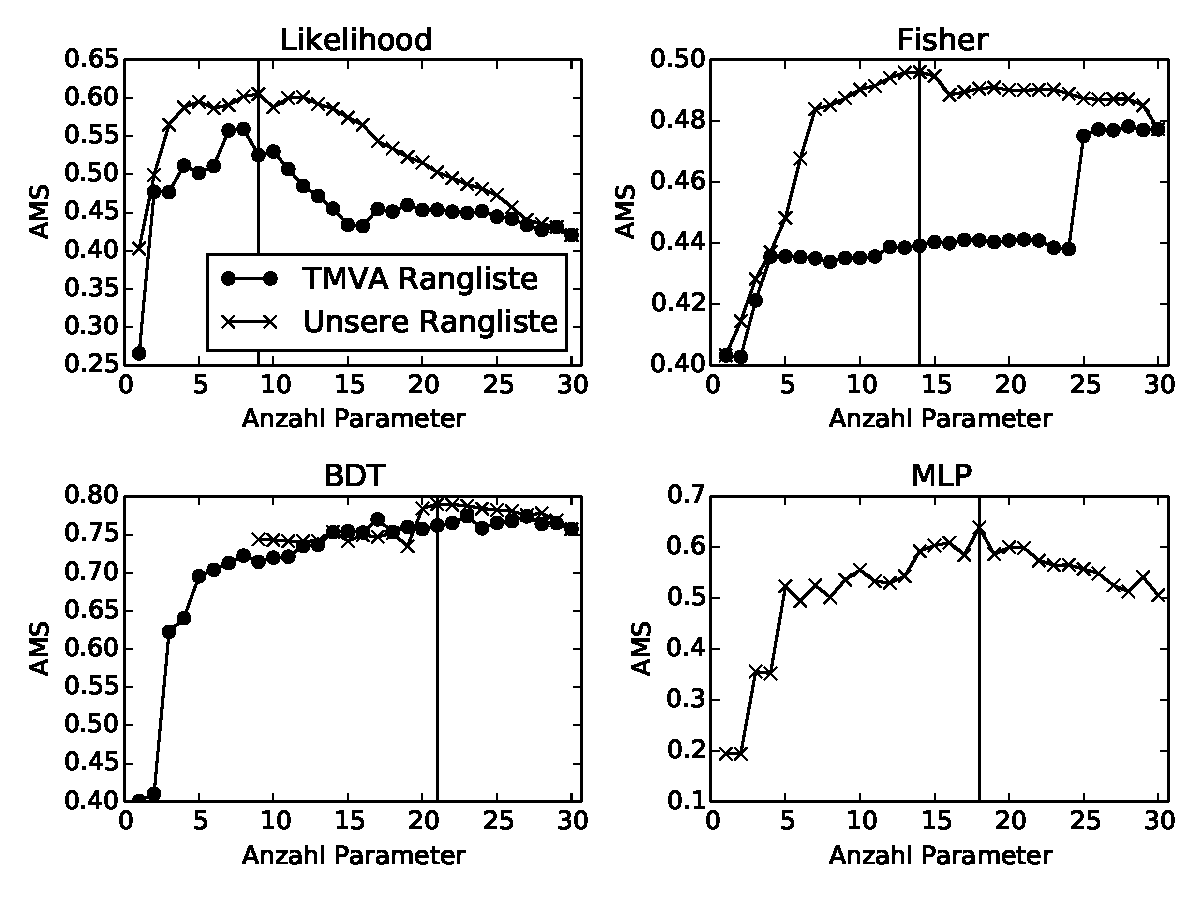
\includegraphics[width=\linewidth]{sections/subset_of_parameters/parameter_count_ranking_by_method.pdf}
  \caption[AMS über der Anzahl der Parameter]{AMS über der Anzahl der Parameter.}
  \label{fig:ams_over_parameter_count}
\end{center}
\end{figure}

\begin{table}
\caption{Bewertung der Parameter. Für die einzelnen Methoden nimmt die
Gewichtung der Parameter von oben nach unten ab. Für jede Methode ist durch
\mbox{"`-----"'} gekennzeichnet, welche Parameter nicht mehr verwendet werden.
Bei der BDT-Methode wurde unter den besten acht Parametern kein Ranking mehr
vorgenommen.}
\small
\hspace{-1cm}
\begin{tabular}{c|c|c|c}
Likelihood & Fisher & BDT & MLP \\
\hline
d\_mass\_transverse\_met\_lep & d\_mass\_transverse\_met\_lep & - & p\_jet\_num
\\
d\_mass\_vis & d\_pt\_ratio\_lep\_tau & - & d\_deltaeta\_jet\_jet \\ 
p\_tau\_pt & p\_lep\_pt & - & d\_mass\_MMC \\ 
d\_deltar\_tau\_lep & d\_mass\_vis & - & p\_jet\_leading\_pt \\ 
d\_pt\_ratio\_lep\_tau & d\_deltar\_tau\_lep & - & d\_mass\_transverse\_met\_l \\ 
p\_met & d\_pt\_h & - & p\_jet\_leading\_eta \\ 
p\_lep\_pt & p\_tau\_pt & - & d\_mass\_jet\_jet \\ 
p\_lep\_eta & d\_mass\_jet\_jet & - & p\_jet\_leading\_phi \\ 
d\_mass\_MMC & p\_met & d\_mass\_MMC & d\_pt\_h \\ 
----- & & & \\ 
p\_jet\_leading\_phi & d\_prodeta\_jet\_jet & d\_lep\_eta\_centrality & d\_mass\_vis \\ 
d\_met\_phi\_centrality & p\_jet\_subleading\_pt & p\_jet\_subleading\_phi & p\_jet\_subleading\_phi \\ 
p\_tau\_phi & p\_lep\_phi & p\_tau\_pt & d\_prodeta\_jet\_jet \\ 
p\_met\_phi & d\_mass\_MMC & d\_mass\_vis & p\_jet\_subleading\_pt \\ 
p\_tau\_eta & d\_deltaeta\_jet\_jet & p\_tau\_phi & p\_tau\_pt \\ 
 & ----- & & \\ 
p\_jet\_subleading\_pt & d\_lep\_eta\_centrality & p\_met\_sumet & p\_met\_phi \\ 
d\_pt\_tot & p\_jet\_leading\_phi & p\_lep\_pt & p\_jet\_all\_pt \\ 
p\_jet\_subleading\_eta & p\_jet\_leading\_eta & p\_lep\_phi & p\_met\_sumet \\ 
d\_prodeta\_jet\_jet & d\_sum\_pt & p\_jet\_subleading\_pt & p\_tau\_eta \\ 
 & & & ----- \\ 
p\_jet\_subleading\_phi & p\_jet\_subleading\_eta & p\_jet\_subleading\_eta & p\_met \\ 
p\_met\_sumet & p\_tau\_phi & d\_pt\_tot & d\_met\_phi\_centrality \\ 
d\_deltaeta\_jet\_jet & p\_met\_phi & p\_jet\_subleading\_eta & d\_pt\_ratio\_lep\_tau \\ 
 & & ----- & \\ 
d\_mass\_jet\_jet & p\_jet\_leading\_pt & p\_jet\_subleading\_phi & p\_tau\_phi \\ 
d\_lep\_eta\_centrality & p\_tau\_eta & p\_jet\_subleading\_pt & p\_jet\_subleading\_eta \\ 
p\_lep\_phi & p\_met\_sumet & d\_pt\_h & p\_lep\_phi \\ 
p\_jet\_num & p\_jet\_num & p\_met & d\_pt\_tot \\ 
d\_pt\_h & d\_pt\_tot & d\_prodeta\_jet\_jet & p\_lep\_eta \\ 
d\_sum\_pt & p\_lep\_eta & p\_lep\_pt & d\_sum\_pt \\ 
p\_jet\_leading\_pt & p\_jet\_subleading\_phi & d\_pt\_tot & d\_lep\_eta\_centrality \\ 
p\_jet\_all\_pt & p\_jet\_all\_pt & p\_met\_phi & p\_lep\_pt \\ 
p\_jet\_leading\_eta & d\_met\_phi\_centrality & p\_lep\_phi & d\_deltar\_tau\_lep

\end{tabular}
\label{table:parameter_ranking}
\end{table}
\section{Transformation der Eingabevariablen}

\subsection{Vorgehen}
Gemäß der Aufgabenstellung in der Template-Datei, experimentierten wir mit den
Transformationen "`Decorrelate"' (D), "`Gauß"' (G), und "`Normalise"' (N).
Um heraus zu finden, ob sie einen Einfluss auf das Ergebnis haben, wendeten wir
sie in allen Kombinationen und Reihenfolgen auf den Input an und evaluierten den AMS-Wert. Evaluiet wurden die Fisher- und die BDT-Methode mit der Untermenge an Variablen, die gemäß Abschnitt \ref{sec:subset_of_variables} ermittelt wurden. 

\subsection{Auswertung}
Die Ergebnisse zeigt Abbildung \ref{fig:ams_over_transforamtion}. Man sieht, dass es für die Fisher-Methode Sinn macht, die Daten zu dekorrelieren
und zu Normalisieren. Die Reihenfolge hat keine Auswirkungen. Bei der
BDT-Methode verschlechtern die Transformationen das Ergebnis. Außerdem gab es
bei dieser Methode bei der Dekorrelation einen Programmfehler, den wir
nicht weiter untersuchten. In Abbildung \ref{fig:ams_over_transforamtion}
sind nur die erfolgreichen Abläufe der BDT-Methode gelistet und deshalb weniger
als bei der Fischer-Methode.


%\usepackage{graphics} is needed for \includegraphics
\begin{figure}[htp]
\begin{center}
  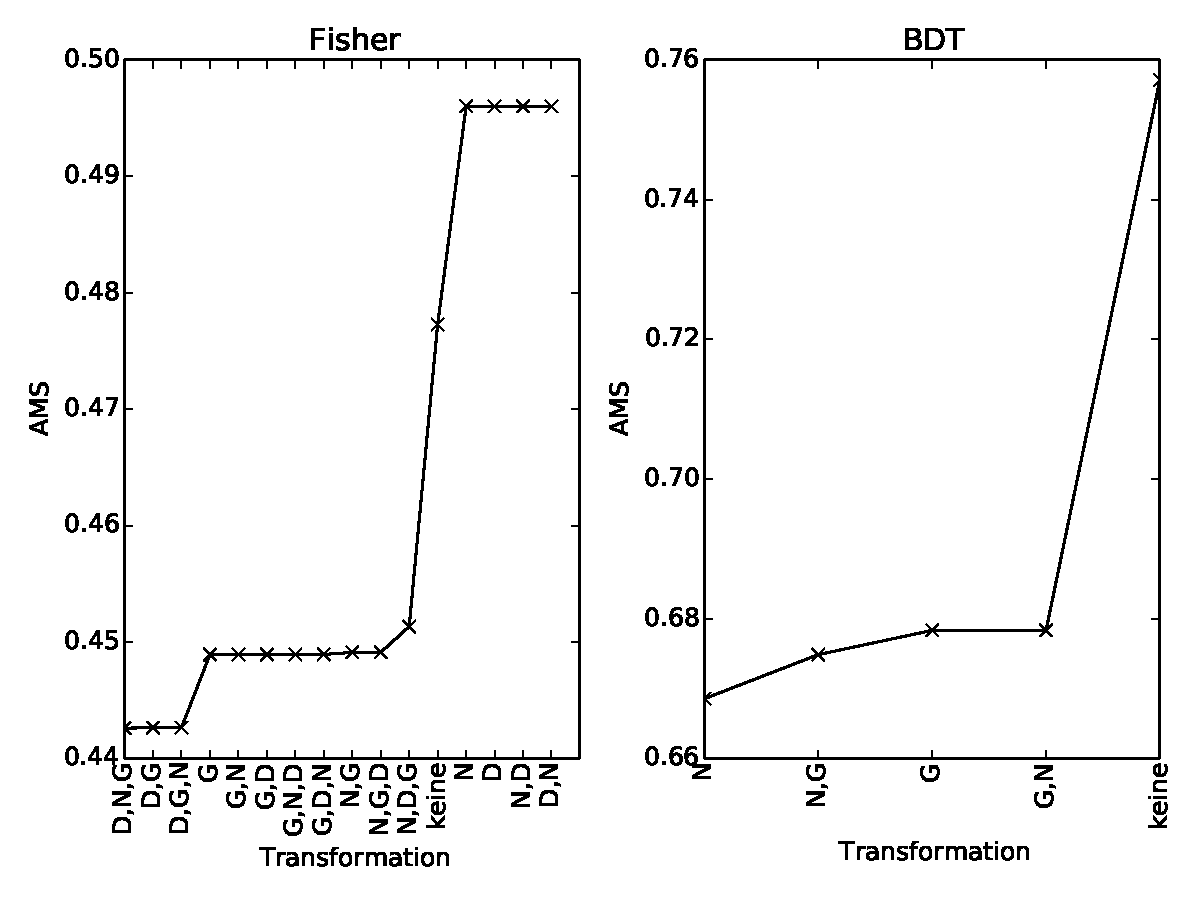
\includegraphics[width=\linewidth]{sections/input_transformations/var_transform_ranking.pdf}
  \caption[AMS über Transformationen der Eingabevariablen]{AMS über Transformationen der Eingabevariablen. Die Buchstaben stehen für "`Decorrelate"' (D), "`Gauß"' (G), und "`Normalise"' (N). Die Transformationen wurden in der Reihenfolge ausgeführt, wie die Buchstaben von unten nach oben gelistet sind.}
  \label{fig:ams_over_transforamtion}
\end{center}
\end{figure}


\section{Optimierung der Parameter des Fisher-Algorithmus}
Um einen höheren AMS-Wert zu erreichen, variierten wir folgende zwei Parameter des Fisher-Algorithmus.
\begin{equation}
\begin{split}
 \mbox{\textit{PDFInterpolMVAPdf}} &\in \{ \mbox{ Spline1,  Spline2, Spline3}  \}  \\
 \mbox{\textit{NsmoothMVAPdf}} &\in \{ \mbox{5,10,15, \ldots, 195} \}
\end{split}
\end{equation}
Der erste Parameter steht für den Grad der Splines mit denen die Wahrscheinlichkeitsverteilungen der Eingabeparameter interpoliert werden. Der zweite Parameter steht für die Anzahl an iterativen Glättungen dieser Verteilungen. 
Das Training dieser Methode mit dem gegebenen Datensatz kostet wenig Zeit - meistens weniger als Minute. Das macht es möglich mit einem brute-force-Ansatz alle Parameterkonstellationen durchzuprobieren. Der AMS-Wert war unabhängig von der Wahl der Parameter \textit{PDFInterpolMVAPdf} und \textit{NsmoothMVAPdf} konstant 0.496. Wir verzichteten auf weitere Optimierungen unter Verwendung des Fisher-Algorithmus, da die erzielten AMS-Werte deutlich unter denen der BDT-Methode lagen.
\section{Optimierung der Parameter der Likelihood-Methode}
Um den AMS-Wert zu erhöhen, wurden drei der Parameter der Likelihood-Methode innerhalb folgender Grenzen variiert:

\begin{equation}
\begin{split}
\mbox{\textit{PDFInterpol}} &\in \{ \mbox{ Spline0,  Spline1, \ldots, Spline5}  \}  \\
 \mbox{\textit{NSmooth}} &\in \{ \mbox{0, 1, \ldots, 12} \} \\
  \mbox{\textit{NAvEvtPerBin}} &\in \{ \mbox{38, 39, \ldots, 52} \} \\
\end{split}
\end{equation}

Die Verteilung der erzielten AMS-Werte ist  Abbildung \ref{fig:likelihood_hist} zu entnehmen.
Da auch bei diesem Verfahren die erzielten AMS-Werte deutlich unter $0,5$ blieben, entschieden wir uns dafür, auch diesen Algorithmus in der weiteren Analyse nicht weiter zu verwenden.


\begin{figure}[htp]
\begin{center}
  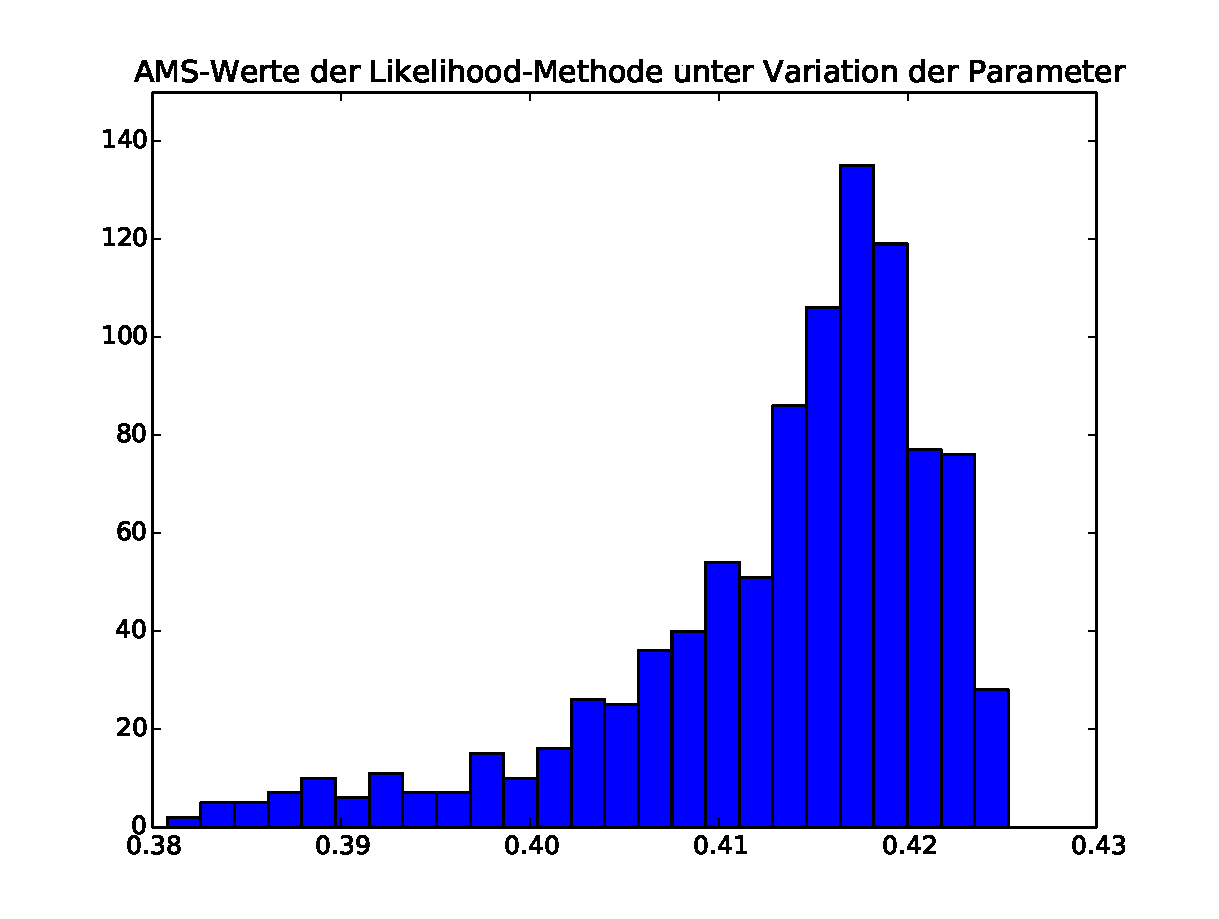
\includegraphics[width=0.7\linewidth]{sections/parameter_optimization_likelihood/likelihood_AMS_hist.pdf}
 \caption[Histogramm der erzielten AMS-Werte]{Histogramm der erzielten AMS-Werte.}
\label{fig:likelihood_hist}
\end{center}
\end{figure}
\section{Optimierung der Parameter des BDT-Algorithmus}
\label{sec:bdt_optimization}
Bei der BDT-Methode wurde je nach Parameter-Konstellation der AMS schlechter wenn nicht der volle Eingabevariablensatz verwendet wurde. Daher wurde der volle Satz an Variablen verwendet. Um die optimalen Parameter für den BDT zu finden, haben wir für die Parameter
\begin{itemize}
	\item NTrees
	\item NEventsMin
	\item Shrinkage
	\item nCuts
	\item MaxDepth
\end{itemize} 
sinnvolle Bereiche festgelegt und suchten in diesem Parameterraum den besten AMS. Da die Laufzeit des Trainings für jeden Punkt im Parameterraum in der Größenordnung von Minuten liegt und wir 5 Parameter haben, lassen sich herkömmliche Optimierungsalgorithmen nicht sinnvoll anwenden.\\
Um einen Überblick zu erhalten ob es gewisse Bereiche im Parameterraum gibt, in denen der AMS generell besser ist, haben wir 1389 mal zufällige Parameter gewählt und den AMS dazu gespeichert. Wenn ein neuer Bestwert erreicht wurde, wurden die kontinuierlichen Parameter NEventsMin und Shrinkage gaußverteilt um die zugehörigen Werte erzeugt.\\
Wie in den Abbildungen \ref{fig:AMS-distribution-plots} (a)-(e) zu erkennen ist, gibt es für einzelne Parameter keinen optimalen Wert. Die Auswirkungen der Parameter sind korreliert und eine Optimierung in nur einem Parameter nicht möglich. Des besten AMS erreichten wir mit
\begin{itemize}
	\item NTrees = 167
	\item NEventsMin = 7.28244760204
	\item Shrinkage = 0.0530833026321
	\item nCuts = 275
	\item MaxDepth  = 9  ,
\end{itemize} 
was auf den Trainingsdaten zu einem AMS-Wert von $0{,}773$ führte.

\begin{figure}[!t]
  \begin{tabular}[b]{cc}
	  \begin{subfigure}[b]{0.5\linewidth}
	   	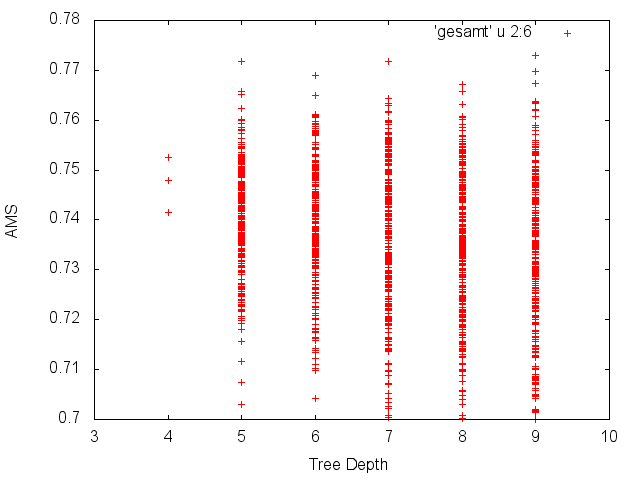
\includegraphics[width=\linewidth]{sections/parameter_optimization_bdt/Depth.png}
 		\caption[]{}
		\label{fig:bdt_Depth}
  	  \end{subfigure} &
  	  \begin{subfigure}[b]{0.5\linewidth}
  	  	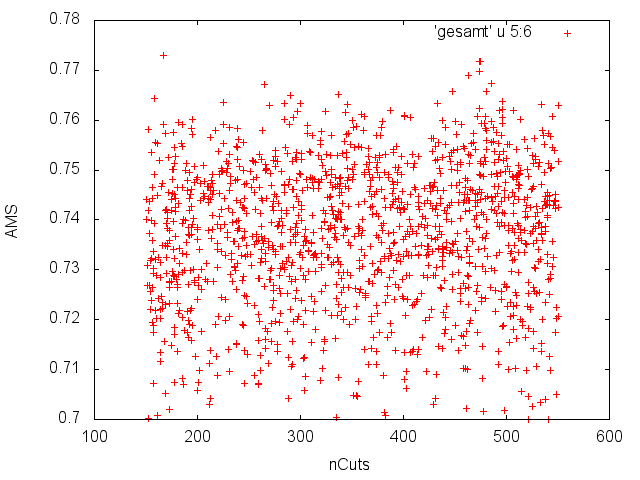
\includegraphics[width=\linewidth]{sections/parameter_optimization_bdt/nCuts.png}
 		\caption[]{}
		\label{fig:bdt_nCuts}
  	  \end{subfigure} \\
  	  
  	  \begin{subfigure}[b]{0.5\linewidth}
	   	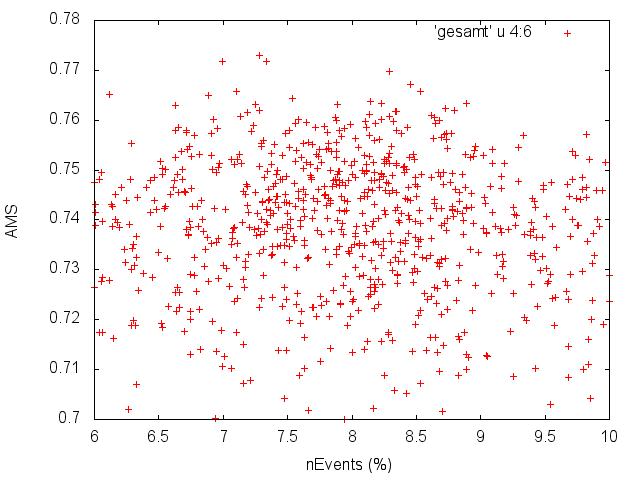
\includegraphics[width=\linewidth]{sections/parameter_optimization_bdt/nEvents.png}
 		\caption[]{}
		\label{fig:bdt_nEvents}
  	  \end{subfigure} &
  	  \begin{subfigure}[b]{0.5\linewidth}
  	  	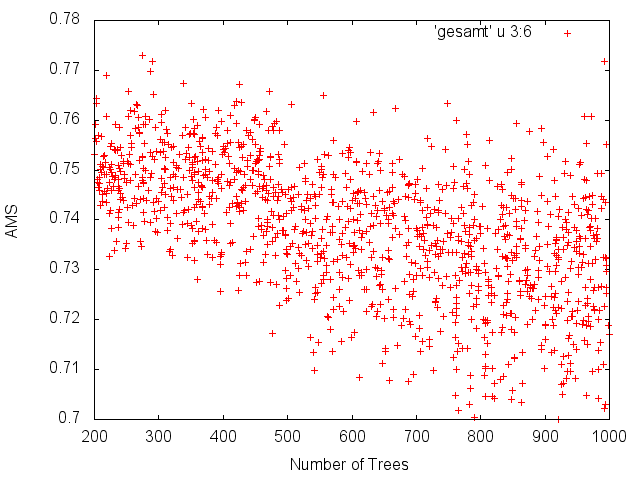
\includegraphics[width=\linewidth]{sections/parameter_optimization_bdt/Nt.png}
 		\caption[]{}
		\label{fig:bdt_Nt}
  	  \end{subfigure} \\
  	  
  	  \begin{subfigure}[b]{0.5\linewidth}
	   	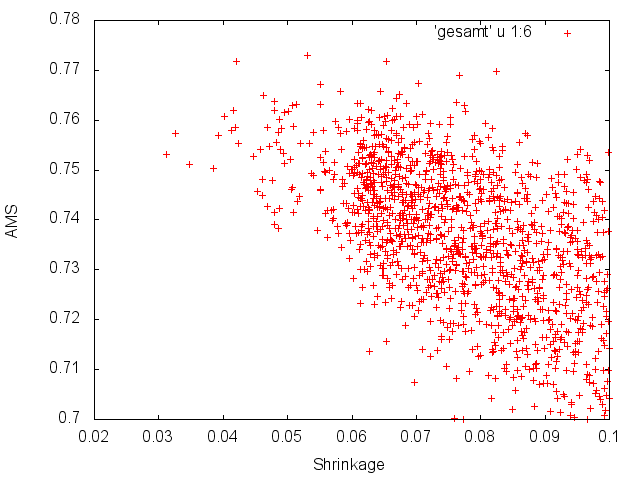
\includegraphics[width=\linewidth]{sections/parameter_optimization_bdt/Shrinkage.png}
 		\caption[]{}
		\label{fig:bdt_Shrinkage}
  	  \end{subfigure} &
  \end{tabular}
  \caption[AMS-Werte für die Parameter der Boosted Decision Trees]{AMS-Werte für die Parameter der Boosted Decision Trees als Scatter-Plots. Jeder Punkt entspricht einem Training.}
  \label{fig:AMS-distribution-plots}
\end{figure}
\section{Optimierung der Parameter des Neuronalen Netzes}
Als (künstliches) Neuronales Netz wird im Allgemeinen jede Annsammlung von verbundenen Neuronen bezeichnet, die ein individuelles Ansprechverhalten zu einem gegebenen Input Signal aufweisen. Das Neuronale Netz besteht meist aus mehreren Schichten, wobei die erste von Input Neuronen und die letzte die Output Neuronen darstellen. In unserem Fall besteht das Output-layer aus lediglich einem Neuron, da nur zwishcen Signal und Background unterschieden werden muss.\\ \\
Um die Zeit zu verringern, die das NN benötigt um die Daten zu trainieren, wurde mit der Option Sampling=0.X gearbeitet welche nur den X-ten Anteil der Trainings- und Testdatensätze verwendet. Zwar muss man dadurch einen etwas schlechteren AMS-Wert in Kauf nehmen, die Laufzeit verringert sich jedoch enorm. Das Sampling wurde benutzt um den Parameter NCycles und die Anzahgl der Hiddenlayers zu optimieren. Eine Variation dieser Paramter hatte allerdings eine recht marginale Auswirkung auf den AMS, wie sich im Folgenden zeigen wird. Außerdem konnte aufgrund der langen Laufzeit nicht wahllos beliebig viele Parameterkonfigurationen ausprobiert werden.\\ \\
Zunächst wurde bei den festen Parametern NCycles = 100,400,700,1000 der Parameter HiddenLayer =N+5,N zu HiddenLayer =N+5,N variiert (siehe Abb xyz). Es stellte sich heraus, dass die N+5,N layer Architektur minimal besser abschnitt. \\ \\
Um das Verhalten bei großen Anzahlen von Zyklendurchläufen zu untersuchen wurde zusätzlich bei Sampling=0.6 die Cycles=650,750,800,5000,10000 ausgewertet (siehe Abb xzy). Eine signifikante Erhöhung der Cycle Anzahl hatte zwar eine rießige Laufzeitverlängerung zur Auswirkung, aber keine Verbesserung des AMS; im Gegenteil dieser hatte sich sogar minimal verschlechtert. \\ \\
Im Folgenden wurde der Bereich um Cycles = 700 näher untersucht, da vermutetr wird dass dort der AMS am besten ist. Hierzu wurden die Cycles =800, 780, 760, 740, 720, 700, 680 mit einem Sampling=0.6 simuliert (Abb. blabla). Da diese Abbildung noch keinen Schlussfolgerungen zulässt wurde in dem darauffolgenden Schritt die Stepsize der cycles verringert und erneut ausgewertet (dieses Mal unter Verwendung des vollen Trainings- und Testdatensatzes, Sampling =False) (siehe Abb sssds). Es stellte sich heraus, dass der AMS bei NCycles $\approx$640 den größten Wert von 0.6215 annimmt. Da dieser Wert jedoch bei Weitem nicht mit dem des BDT mithalten kann, wurde das NN als Methode verworfen. \\ \\
\section{Fazit und unser Score}
Für die Analyse des kompletten Datensatzes verwendeten wir die BDT-Methode mit dem Parametersatz, der die besten Trainingswerte erreichte. (siehe Abschnitt \ref{sec:bdt_optimization}) Die Eingabevariablen wurden nicht transformiert und der volle Variablensatz wurde verwendet. Der erreichte AMS-Wert liegt bei
\begin{equation}
2.54
\end{equation}

\begin{figure}[htp]
\begin{center}
  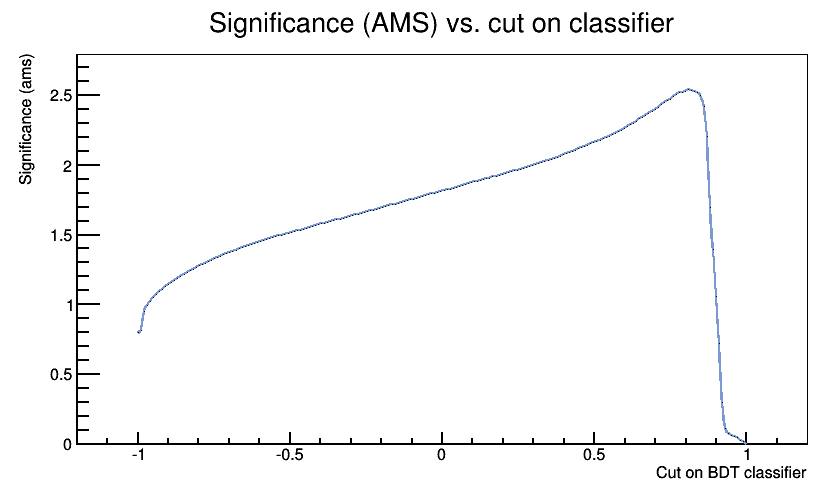
\includegraphics[width=0.7\linewidth]{sections/conclusion/AMS_vs_Cut_cropped.png}
 \caption[]{}
\label{fig:bdt_Shrinkage}
\end{center}
\end{figure}
%\bibliography{bibliography}
\bibliographystyle{alpha}
%\bibliographystyle{unsrt}

\end{document}
